\section{Gaussian Mixture Models and Cell Reconstruction}
\label{sec:gmm-gmm}
Data that form \emph{clusters} in feature space, \ie regions with a dense accumulation of
data points, can be meaningfully interpreted as data generated by a distribution with multiple
local maxima, which, in turn, can be modeled by a convex combination of simpler, single-mode distributions.

\begin{mydef}
    \label{def:convex-combination}
    A \emph{convex combination} of points $\{x_h\}_{h=1,\hdots,H}$ is a linear combination of points
    $\{x_h\}_{h=1,\hdots,H}$ with non-negative weights $\{\alpha_h\}_{h=1,\hdots,H}$ that sum up to $1$ (normalization):
    \begin{align}
        \label{eq:def-convex-combination}
        &\sum_{h=1}^H \alpha_h x_h, \\
        &\alpha_h \ge 0 \; \forall h \wedge \sum_{h=1}^H \alpha_h = 1.
    \end{align}
\end{mydef}
For clarification, the convex combination of the unit coordinate vectors in three dimensions is visualized in
\cref{fig:gmm-convex-combination}.
\begin{figure}
    \centering
    \tdplotsetmaincoords{60}{110}

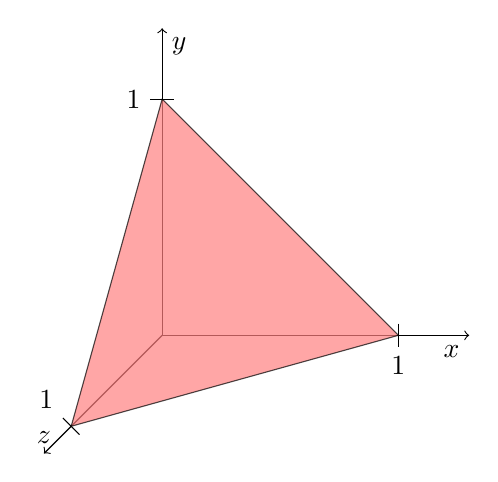
\begin{tikzpicture}[scale=3]
    \begin{scope}
        \draw[->] (0,0,0) -- (1.3,0,0) node[anchor=north east]{$x$};
        \draw[->] (0,0,0) -- (0,1.3,0) node[anchor=north west]{$y$};
        \draw[->] (0,0,0) -- (0,0,1.3) node[anchor=south]{$z$};
        \draw [fill=red!50, opacity=0.7] (0,0,1)--(1,0,0)--(0,1,0)--cycle;
        \draw (1,0.05,0) -- (1,-0.05,0) node[anchor=north]{$1$};
        \draw (0.05,1,0) -- (-0.05,1,0) node[anchor=east] {$1$};
        \draw (0.035,-0.035,1) -- (-0.035,0.035,1) node[anchor=south east]{$1$};
        
    \end{scope}
\end{tikzpicture}

%%% Local Variables: 
%%% mode: latex
%%% TeX-master: "../../main"
%%% End: 

    %\rule{\textwidth}{0.3pt}
    \caption[Convex sum visualization]{A visualization of the convex sum of unit vectors in a three dimensional coordinate
        system: The red area (including the boundary) is the feasible region for the convex combination.}
    \label{fig:gmm-convex-combination}
\end{figure}

\cref{def:convex-combination} allows for definition of \emph{mixture models} in terms of convex
combinations.
\begin{mydef}[{{\citealp[Chapter~20]{barber_12_bayesian}; \citealp[Chapter~9]{bishop_07_pattern};
            \citealp{mclachlan_00_finite}}}]
    \label{def:mixture-model}
    A convex combination of distributions\footnote{The term ``distribution'' here refers to probability density~\citep[158]{barber_12_bayesian}.}
    \begin{align}
        \label{eq:gmm-distribution}
        p(v) = \sum_{h=1}^Hp(v|h)p(h)
    \end{align}
    is called a \emph{mixture model}.
\end{mydef}
The \emph{visible} variable $v$ corresponds to a data sample. The distribution is a sum of $H$
component models $p(v|h)$ weighted by $p(h)$, which corresponds to the weight $\alpha_h$ in
\cref{eq:def-convex-combination}. The weight can be interpreted as the prior probability of the data
sampled being generated by a particular component $h$, representing cluster $h$, as the definition
of a convex combination fulfills the requirements of a discrete probability distribution, namely
non-negativity and normalization. The data generation process follows a two step procedure: First, a
component distribution index $h$ is sampled from $p(h)$. Then, a data point is sampled from
$p(v|h)$. $h$ is called a \emph{hidden} variable.

In a \emph{Gaussian mixture model}, the data follow a convex sum of multivariate Gaussian distributions,
\begin{align}
    \label{eq:gmm-normal}
    p(v|h) &= \mathcal{N}({v}|\MUH , \SIGMAH ) \\ 
    &= \frac{1}{\sqrt{\det(2\pi\SIGMAH )} }\exp\left(-\frac{1}{2}({v}-\MUH )^\intercal
        \left(\SIGMAH\right) ^{-1} ({v}-\MUH )\right),
\end{align}
with mean $\MUH$ and covariance matrix $\SIGMAH$ for each component $h$. In general,
\begin{align}
    z\sim\mathcal{N}(z|\mu, \Sigma)
\end{align}
denotes that variable $z$ follows a normal distribution with
mean $\mu$ and covariance $\Sigma$. For brevity,
\begin{align}
    \label{eq:gmm-theta}
    \Theta &= \left\{\THETAH\right\}_{h=1,\hdots ,H}, \\
    \THETAH &= \left\{\MUH, \SIGMAH\right\}
\end{align}
refer to all parameters of the $h$-th component of the Gaussian mixture model. The parameters
\begin{align}
    \label{eq:gmm-pi}
    \Pi &= \left\{\pi_h\right\}_{h = 1, \hdots , H}, \\
    p(h) &= \pi_h \; \forall h \label{eq:gmm-pi-2}
\end{align}
define the discrete probability distribution to weigh the cluster components. \cref{fig:gmm-example}
shows data sampled from two Gaussian distributions and a GMM fit to the data.

\newsavebox{\covmatfirst}% Box to store smallmatrix content
\savebox{\covmatfirst}{$\left(\begin{smallmatrix}\hfill 5.25&\hfill 1.575\\\hfill 1.575&\hfill 3.5\end{smallmatrix}\right)$}
\newsavebox{\covmatsecond}% Box to store smallmatrix content
\savebox{\covmatsecond}{$\left(\begin{smallmatrix}\hfill 2.8&\hfill 1.75\\\hfill 1.75&\hfill 5.95\end{smallmatrix}\right)$}
\newsavebox{\predmatfirst}% Box to store smallmatrix content
\savebox{\predmatfirst}{$\left(\begin{smallmatrix}\hfill 5.16&\hfill 1.53\\\hfill 1.53&\hfill 3.41\end{smallmatrix}\right)$}
\newsavebox{\predmatsecond}% Box to store smallmatrix content
\savebox{\predmatsecond}{$\left(\begin{smallmatrix}\hfill 2.86&\hfill 1.87\\\hfill 1.87&\hfill 5.89\end{smallmatrix}\right)$}

\begin{figure}
    \centering
    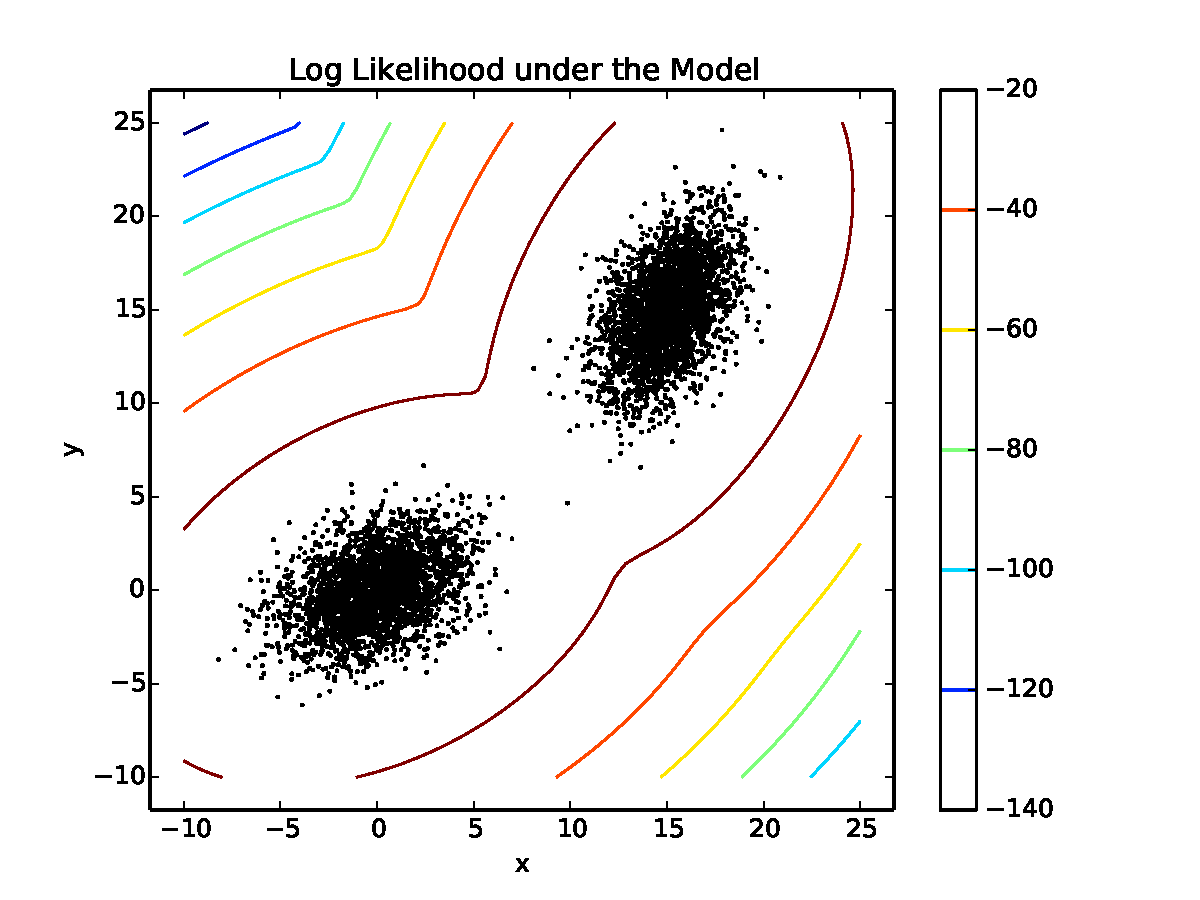
\includegraphics[width=0.7\textwidth]{images/gmm/gmm_example.pdf}
    %\rule{\textwidth}{0.3pt}
    \caption[GMM example]{\protect The black circles are data points sampled from two normal distributions with
        $\mu_1=(0,0)^\intercal$,$\Sigma_1=$\usebox{\covmatfirst} and
        $\mu_2=(15,15)^\intercal$,$\Sigma_2=$\protect\usebox{\covmatsecond}. 3000 samples are taken from
        each distribution. The GMM fit is represented by colored contour lines that represent levels
        of equal observation log likelihood. The predicted parameters are $\mu_1^{pred}=(-0.03,
        0.02)^\intercal$,$\Sigma_1^{pred}=$\protect\usebox{\predmatfirst}, $\mu_2^{pred}=(15.02,
        14.99)^\intercal$,$\Sigma_2^{pred}=$\protect\usebox{\predmatsecond}. The prior probabilities are in
        accord with the data generation process $\pi_1 = \pi_2 =
        0.500$.}
        % Scikit-learn~\cite{scikit-learn} and Matplotlib~\cite{hunter_07_matplotlib} were
        % used to create this plot.
        % $\sigma_1=\left(
        %     \begin{smallmatrix}
        %         1.5 &-0.9 \\
        %         0 & 1
        %     \end{smallmatrix}
        %     \right)$
    \label{fig:gmm-example}
\end{figure}

For $N$ independent and
identically distributed (\emph{iid}) random variables $\{v^n\}_{n=1,\hdots ,N}$, a Gaussian mixture model takes the form
\begin{align}
    \label{eq:gmm-iid}
    p(v^1,\dots ,v^N, h^1, \dots ,h^N) = \prod_{n=1}^N p(v^n|h^n)p(h^n).
\end{align}
Here, $h^n \in \{1,\hdots ,H\}$ means that the $n$-th data sample is assigned to cluster $h^n$.  A
graphical representation of this distribution is shown in \cref{fig:gmm-gm-plate} using the plate
notation:
\begin{mydef}
    In the visual representation of graphical models, \emph{plate notation} refers to grouping
    variables into a subgraph by enclosing them in a rectangle (plate). The number on the plate is
    the number of repetitions or duplications of that subgraph.
\end{mydef}
An illustrative example for plate notation is given in \cref{fig:gmm-plate-expl}.
\begin{figure}
    \centering
    \begin{subfigure}[t]{0.48\textwidth}
        \centering
        \begin{tikzpicture}[baseline=0pt]
    \begin{scope}
        \node[main, label=below:$v_1$, fill=black!30] (v) {};
        \node[main, label=below:$v_2$, fill=black!30, above of=v] (v1) {};
        \node[main, label=below:$v_3$, fill=black!30, below of=v] (v2) {};
        \node[main, label=below:$h$, left of=v, xshift=-10] (h) {};
        \path (h) edge[connect] (v);
        \path (h) edge[connect] (v1);
        \path (h) edge[connect] (v2);
    \end{scope}
\end{tikzpicture}


%%% Local Variables: 
%%% mode: latex
%%% TeX-master: "../../main"
%%% End: 

        \caption{Directed Acyclic Graph}
        \label{fig:gmm-plate-expl-dag}
    \end{subfigure}
    ~
    \begin{subfigure}[t]{0.48\textwidth}
        \centering
        \begin{tikzpicture}[baseline=0pt]
    \begin{scope}
        \node[main, label=below:$v$, fill=black!30] (v) {};
        \node[main, label=below:$h$, left of=v, xshift=-10] (h) {};
        \node[main, fill=black!30, below of=v, color=black!0] (v2) {};
        \node[rectangle, inner sep=5mm,draw=black!100, fit= (v)] (r) {};
        \node[anchor=south east,inner sep=1pt] at (r.south east) {$3$};
        \path (h) edge[connect] (v);
        %%%% DIRTY HACK TO ALLOW FOR CAPTIONS BEING ON THE SAME HEIGHT!!
        %%%% MAYBE RECONSIDER!!
        \node[main, label=below:{\color{white} 1}, color=black!0, fill=black!0, below of=v] (v2) {};
    \end{scope}
\end{tikzpicture}

%%% Local Variables: 
%%% mode: latex
%%% TeX-master: "../../main"
%%% End: 

        \caption{Plate Notation}
        \label{fig:gmm-plate-expl-plate}
    \end{subfigure}
    %\rule{\textwidth}{0.3pt}
    \caption[Plate notation example]{Plate notation example: The distribution $p(v_1,v_2,v_3,h) =
        p(v_1|h)p(v_2|h)p(v_3|h)p(h)$ is represented by a directed acyclic graph
        (\subref{fig:gmm-plate-expl-dag}). The plate notation for the same graph in
        (\subref{fig:gmm-plate-expl-plate}) is much  more compact.}
    \label{fig:gmm-plate-expl}
\end{figure}
The observation likelihood for given data can be derived by marginalizing over \cref{eq:gmm-iid}:
\begin{align}
    \label{eq:gmm-obs-likelihood}
    p(v^1,\hdots ,v^N) = \prod_{n=1}^N\sum_{h^n=1}^Hp(v^n|h^n)p(h^n).
\end{align}
For the application of GMMs in the context of conservation tracking, it is mandatory to infer the
cluster a data point belongs to. This can be achieved by maximizing the conditional probability
\begin{align}
    \label{eq:gmm-assign-clusters}
    \left\{ h_{\max }^n\right\}_{n=1,\hdots ,N} = &\argmax_{ h^1, \hdots ,h^N} p(h^1, \dots ,h^N|v^1,
    \hdots ,v^N) \\
    = & \left\{ \argmax_{h^n} p(h^n|v^n) \right\}_{n=1,\hdots ,N}.
\end{align}
The second equality holds due to the factorization of the distribution.  For this operation, the
model parameters $\Theta$ and $\Pi$ as defined in \crefrange{eq:gmm-theta}{eq:gmm-pi-2} need to be determined first, which
requires a formulation of the distribution that explicitly shows the dependency on the model
parameters:
\begin{align}
    \label{eq:gmm-distr-param}
    p(v^1,\dots ,v^N,h^1,\dots h^N|\Theta ,\Pi ) = \prod_{n=1}^Np(v^n|h^n, \Theta )p(h^n|\Pi )
\end{align}
The optimal parameters
\begin{align}
    \label{eq:gmm-ml}
    \left\{\Theta_{opt} ,\Pi_{opt}\right\} &= \argmax_{\Theta ,\Pi } p\left(v^1,\hdots ,v^N|\Theta
        ,\Pi\right) \\
    &= \argmax_{\Theta ,\Pi } \prod_{n=1}^Np\left(v^n|\Theta ,\Pi\right)
\end{align}
are then inferred by maximum likelihood. The commonly-used method for maximizing the likelihood of a
mixture model is the \emph{expectation maximization} (EM) algorithm, an iterative procedure, that in
many cases, including Gaussian mixture models, results in simple update formulae for the model
parameters. In general, the EM algorithm consists of an iterative repetition of two steps, namely the
\begin{itemize}
      \item \textbf{E-step} that maximizes the likelihood for the current set of parameters, \ie -- in
    the case of clustering -- assigning the data points to the correct clusters, and the
      \item \textbf{M-step} that -- given the assignments from the E-step -- estimate the parameters
    of the distribution.
\end{itemize}
These two steps are repeated until convergence or an iteration threshold. In general and in
particular for the Gaussian mixture models, the likelihood
is not a convex function. Therefore, the EM algorithm might get stuck in local minima and the result
can vary depending on the initial parameters. Detailed explanations of the EM algorithm can be
found in \citep[Chapter~11.2]{barber_12_bayesian},
\citet[Chapter~3]{mclachlan_97_em} and \citet{borman_04_expectation}.

The update equations for EM on a Gaussian mixture models are:
\begin{align}
    \label{eq:gmm-update-eq}
    \MUH_{\text{new}} &= \sum_{n=1}^Np_{\text{old}}\left(v^n|h\right)v^n, \\
    \SIGMAH_{\text{new}} &=
    \sum_{n=1}^Np_{\text{old}}(v^n|h)\left(v^n-\MUH\right)\cdot\left(v^n-\MUH\right)^\intercal, \\
    p_{\text{new}}(h) &= \frac{1}{N}\sum_{n=1}^N p_{\text{old}}\left(h|v^n\right).
\end{align}
These update rules ensure that $\SIGMAH$ is symmetric positive semidefinite, which is a requirement
for any covariance matrix.



\begin{figure}
    \centering
    % \begin{tikzpicture}
% \tikzstyle{main}=[circle, minimum size = 10mm, thick, draw =black!80, node distance = 16mm]
% \tikzstyle{hyparam}=[rectangle, minimum size = 5mm, thick, draw =black!80, fill = black!10, node distance = 16mm]
% \tikzstyle{param}=[rectangle, minimum size = 5mm, thick, draw =black!80, node distance = 16mm]
% \tikzstyle{connect}=[-latex, thick]
% \tikzstyle{selector}=[-latex, -|, snake=snake,segment amplitude=.4mm,segment length=2mm,line after snake=1mm, thick]
% \tikzstyle{shortconnect}=[-latex, thin]
% \tikzstyle{box}=[rectangle, draw=black!100]
% \tikzstyle{switch}=[circle, minimum size = 1mm, fill = black!100, draw=black!100]
%   \node[param] (phi) [label=below:$p(h)$] {$[H]$};
%   \node[main] (z) [right of=phi,label=below:$h^n$] {K};
%   \node[param] (mu) [above of=phi,yshift=10mm, label=below:$\MUH$] { };
%   \node[main, fill = black!10] (x) [right of= z,label=below:$v^n$] { };
%   \node[param] (sigma) [above of=z,yshift=10mm, label=right:$\SIGMAH$] { };
%   \path (phi) edge [connect] (z)
%         (z) edge [selector] (x)
%         (mu) edge [connect] (x)
%         (sigma) edge [connect] (x);
%   \node[rectangle, inner sep=0mm, fit= (z) (x),label=below right:$N$, xshift=9mm] {};
%   \node[rectangle, inner sep=4.4mm,draw=black!100, fit= (z) (x), xshift=1mm] {};
%   \node[rectangle, inner sep=2mm, fit= (mu) (sigma),label=below right:$H$, yshift=-2mm, xshift=11mm] {};
%   \node[rectangle, inner sep=6.4mm,draw=black!100, fit= (mu) (sigma), yshift=-2mm, xshift=3mm] {};
% \end{tikzpicture}

\begin{tikzpicture}
  \node[param] (pi) [] {$\Pi$};
  \node[main] (z) [right of=pi,label=below:$h^n$] { };
  \node[param] (mu) [above of=pi,yshift=10mm, label=below:$\MUH$] { };
  \node[main, fill = black!30] (x) [right of= z,label=below:$v^n$] { };
  \node[param] (sigma) [above of=z,yshift=10mm, label=right:$\SIGMAH$] { };
  \path (pi) edge [connect] (z)
        (z) edge [connect] (x)
        (mu) edge [connect] (x)
        (sigma) edge [connect] (x);
  \node[rectangle, inner sep=0mm, fit= (z) (x),label=below right:N, xshift=9mm] {};
  \node[rectangle, inner sep=4.4mm,draw=black!100, fit= (z) (x), xshift=1mm] {};
  \node[rectangle, inner sep=2mm, fit= (mu) (sigma),label=below right:H, yshift=-2mm, xshift=11mm] {};
  \node[rectangle, inner sep=6.4mm,draw=black!100, fit= (mu) (sigma), yshift=-2mm, xshift=3mm] {};
\end{tikzpicture}



%%% Local Variables: 
%%% mode: latex
%%% TeX-master: "../../main"
%%% End: 

    %\rule{\textwidth}{0.3pt}
    \caption[GMM: Directed acyclic graph representation]{Directed acyclic graph representation of a
        Gaussian mixture model (taken and modified from~\cite{wikipedia_12_gmm}): The latent
        variable $h^n$ indicates the component membership of the $n$-th data point and follows the
        discrete probability distribution $p(h)$ with parameters $\Pi$. The associated observation
        $v^n$ is then generated by $p(v^n|h^n)=\mathcal{N}\left(\VEC{v}^n|\VEC{\mu}^{(h^n)} ,
            \VEC{\Sigma}^{(h^n)}\right)$. The shading of the $v^n$ node indicates the observable
        variable. The numbers in the bottom right corners of the plates indicate the number of
        duplications of each plate.}
    \label{fig:gmm-gm-plate}
\end{figure}


\subsection{Reconstructing Cell Identities}
Gaussian mixture models are an outstanding choice for clustering when the number of clusters $H$ in
the data is known. Then, $H$ does not need to be inferred from the data. In the context of
conservation tracking, the number of clusters is readily available as the number of cells per
connected component as determined by the tracking algorithm. Therefore, GMMs are a good choice for
the missing link in the tracking framework. Using them for cell reconstruction advances the
capabilities of the conservation tracking by enabling the reconstruction of tracks that contain
merged objects which would otherwise have been lost.

In a post-processing step a Gaussian mixture is fit to each merger object, \ie a connected component
that contains more than one cell. The coordinates are extracted from the binary segmentation
image.
% In order to avoid unfavorable local minima in the expectation maximization, the means and
% covariances are initialized with the means and covariances from cells in the previous timestep. The
% predicted means are vital for the merger resolution and are injected in a modified subgraph of the
% original hypotheses graph, that contains all reconstructed cells.
%
The following \cref{sec:gmm-hypotheses} contains a detailed description of how GMM clustering
can be utilized for the reconstruction of lost tracks due to merged objects.
%%% Local Variables: 
%%% mode: latex
%%% TeX-master: "../../../main"
%%% End: 
